\documentclass[UTF8,fontset=none,12pt]{ctexart}

\setCJKmainfont{Songti SC}
\setCJKsansfont{PingFang SC}
\setCJKmonofont{Songti SC}

\usepackage[a4paper,margin=2.35cm]{geometry}
\usepackage{amsmath,amssymb,amsthm,mathtools,bm}
\usepackage{graphicx}
\usepackage{float}
\usepackage{booktabs}
\usepackage{array}
\usepackage{enumitem}
\usepackage[hidelinks]{hyperref}

\title{数值线性代数\quad 第 39 讲：双正交化方法}
\author{Lloyd N. Trefethen、David Bau III\\中文阅读版}
\date{}

\begin{document}
\maketitle

\noindent
\textbf{原书页码：}303--312；\quad
\textbf{目标 PDF 页码：}318--327。

对于非对称（更一般地，非 Hermitian）线性系统，并不是所有 Krylov 子空间迭代
都必须使用长度不断增长、代价不断增加的递推。基于三项递推的方法也已经被构造
出来，而且它们是目前最有力的非对称迭代方法。至少对其中一部分方法而言，需要
付出的代价是：必须同时处理两个 Krylov 子空间，而不是一个；这两个子空间分别
由 $A^*$ 和 $A$ 的乘法生成。

\section*{我们目前所处的位置}

在第 31 讲（原书第 245 页）我们给出过 Krylov 子空间矩阵迭代的分类：

\begin{center}
\begin{tabular}{c|c|c}
\toprule
 & $Ax=b$ & $Ax=\lambda x$\\
\midrule
$A=A^*$ & CG & Lanczos\\
\addlinespace
$A\ne A^*$ & GMRES、CGN、BCG 等 & Arnoldi\\
\bottomrule
\end{tabular}
\end{center}

其中三个方框的讨论已经完成；对于左下角的第四个位置 GMRES，我们也已经在前面
讲过。本讲先用很短的篇幅介绍 CGN，再转向本讲的主要主题：右下角
“BCG 等”所代表的双正交化方法。图 39.1 给出了这些方法之间的结构关系。

\begin{figure}[H]
\centering
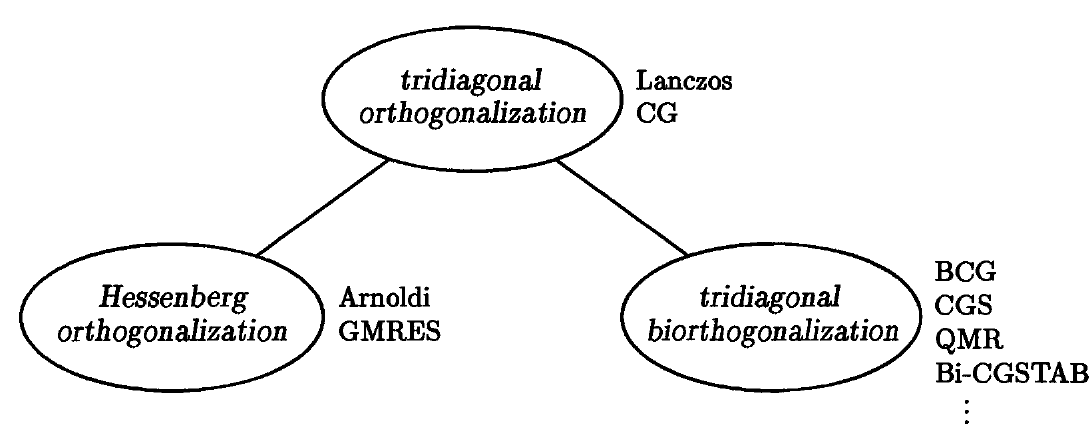
\includegraphics[width=0.92\textwidth]{../assets/figure-39-1-classification.png}
\parbox{0.94\textwidth}{\small 图 39.1. Krylov 子空间迭代的分类。若矩阵是 Hermitian 的（上方一行），
可以用三项递推关系把它正交化为三对角矩阵；若不是 Hermitian 的，就必须在三对角结构
与正交性之间放弃其中一个。图中文字保留原图标注，便于和原书核对。}
\end{figure}

\section*{CGN：把 CG 应用于正规方程}

设 $A\in\mathbb C^{m\times m}$ 非奇异，但不一定是 Hermitian 矩阵。于是对任意
$b\in\mathbb C^m$，方程 $Ax=b$ 都是一个非奇异的方阵系统。求解这类系统的
最简单方法之一，是把 CG 迭代应用于正规方程

\begin{equation}
A^*Ax=A^*b.
\tag{39.1}
\end{equation}

实际计算时不会显式形成 $A^*A$，因为这样需要 $m^3$ 量级的浮点运算。取而代之，
每次计算矩阵--向量乘积 $A^*Av$ 时，分两步先算 $Av$，再算 $A^*(Av)$。
由于 $A$ 非奇异，$A^*A$ 是 Hermitian 正定矩阵；若 $A$ 为实矩阵，则它是对称
正定矩阵。因此第 38 讲中的定理都可以直接使用：只要 $A^*A$ 的特征值分布良好，
就可以期待快速收敛。这一方法称为 CGN（也称 CGNR），大意是
“应用于正规方程的 CG”。

由于 CG 的行为已经分析过，理解 CGN 不需要新的理论。若像算法 38.1 那样取初始
猜测 $x_0=0$，则由定理 38.1，后续迭代属于由 $A^*A$ 生成的 Krylov 子空间：

\begin{equation}
x_n\in\operatorname{span}\bigl\{
A^*b,\,(A^*A)A^*b,\,\ldots,\,(A^*A)^{n-1}A^*b
\bigr\}.
\tag{39.2}
\end{equation}

定理 38.2 告诉我们，在这个子空间上，误差的 $A^*A$-范数在每一步都被最小化。
如果 $e_n=x_* - x_n$、$r_n=b-Ax_n$，那么

\[
\lVert e_n\rVert_{A^*A}^2
=e_n^*A^*Ae_n
=\lVert Ae_n\rVert_2^2
=\lVert r_n\rVert_2^2.
\]

所以这也就是说，残量的 2-范数被最小化：

\begin{equation}
\lVert r_n\rVert_2=\text{最小值}.
\tag{39.3}
\end{equation}

因此，CGN 和 GMRES 一样，都是最小残量方法。不过，它们所使用的 Krylov 子空间
分别是第 33 讲的式（33.5）与式（39.2），两者不同，所以这两个方法绝不等价。

根据定理 38.3，CGN 的收敛由 $A^*A$ 的特征值控制，而这些特征值正好是 $A$
奇异值的平方。因此，CGN 的收敛由 $A$ 的奇异值决定，原则上与 $A$ 的特征值
无关。遗憾的是，这里出现了平方。如果 $A$ 的条件数为 $\kappa$，则 $A^*A$
的条件数为 $\kappa^2$；将第 38 讲的估计改写为 CGN 的形式，得到

\begin{equation}
\frac{\lVert r_n\rVert_2}{\lVert r_0\rVert_2}
\leq
2\left(\frac{\kappa-1}{\kappa+1}\right)^n.
\tag{39.4}
\end{equation}

当 $\kappa$ 很大时，这比第 38 讲的估计糟糕得多：为了达到固定精度，所需迭代步数
是 $O(\kappa)$，而不是 $O(\sqrt{\kappa})$。这种“条件数平方化”使 CGN 名声不佳，
总体而言这或许是有理由的。不过，对某些问题，CGN 仍然会远胜其他方法，因为其他
方法的收敛依赖特征值，而不是奇异值。只要构造一个奇异值表现良好、特征值表现很差
的矩阵即可，例如一个条件良好、但谱在复平面原点周围包围原点的矩阵。

一个极端例子是如下 $m\times m$ 循环矩阵：

\begin{equation}
A=
\begin{bmatrix}
0&1&&&\\
 &0&1&&\\
 &&0&\ddots&\\
 &&&\ddots&1\\
1&&&&0
\end{bmatrix}.
\tag{39.5}
\end{equation}

这个矩阵的所有奇异值都等于 1，但特征值是 $m$ 次单位根。对于一般的右端项 $b$，
GMRES 需要 $m$ 步才能收敛，而 CGN 一步就收敛（见习题 39.1）。

CGN 的另一个优点是：因为它建立在正规方程上，所以可以不加修改地应用于最小二乘
问题，此时 $A$ 不再要求是方阵（参见算法 11.1）。另一种做法是使用习题 19.1
中的块系统（19.4）。

\section*{三对角双正交化}

正如第 36 讲所见，Lanczos 迭代是一个\textbf{三对角正交化}过程。如果在精确算术
下完整运行 $m$ 步，它会把 Hermitian 矩阵酉相似约化为三对角形式：

\[
A=QTQ^*.
\]

如果 $A$ 不是 Hermitian 的，一般不可能得到这样的约化；我们必须放弃酉变换，或者
放弃最终的三对角形式。Arnoldi 迭代是 Hessenberg 正交化过程，它选择放弃后者。
完整运行 $m$ 步时，它把任意方阵酉相似约化为 Hessenberg 形式：

\[
A=QHQ^*.
\]

双正交化方法采取相反的选择：坚持得到三对角矩阵，但放弃酉变换。于是得到
\textbf{三对角双正交化}：

\[
A=VTV^{-1},
\]

其中 $V$ 非奇异，但一般不是酉矩阵（见图 39.1）。对上式取伴随可得等价关系

\[
A^*=V^{-*}T^*V^*,
\qquad
V^{-*}=(V^*)^{-1}=(V^{-1})^*.
\]

“双正交”一词指的是：虽然 $V$ 的列向量彼此不一定正交，但它们与 $V^{-*}$ 的列
向量正交。这直接来自

\[
(V^{-*})^*V=V^{-1}V=I.
\]

为了把这个想法变成迭代算法，考虑 $n<m$ 的情形。设 $V$ 是满足
$A=VTV^{-1}$ 的非奇异矩阵，且 $T$ 为三对角矩阵；令 $W=V^{-*}$。记 $v_j$
和 $w_j$ 分别为 $V$ 与 $W$ 的第 $j$ 列。它们满足双正交关系

\begin{equation}
w_i^*v_j=\delta_{ij},
\tag{39.6}
\end{equation}

其中 $\delta_{ij}$ 是 Kronecker $\delta$ 函数。对 $1\leq n\leq m$，定义
$m\times n$ 矩阵

\begin{equation}
V_n=\begin{bmatrix}v_1&\cdots&v_n\end{bmatrix},
\qquad
W_n=\begin{bmatrix}w_1&\cdots&w_n\end{bmatrix}.
\tag{39.7}
\end{equation}

双正交条件的矩阵形式为

\[
W_n^*V_n=V_n^*W_n=I_n.
\]

这里 $I_n$ 是 $n$ 阶单位矩阵。

\subsection*{关键矩阵关系与三项递推}

双正交化方法的关键公式是

\begin{align}
AV_n&=V_{n+1}\widetilde T_n, \tag{39.8}\\
A^*W_n&=W_{n+1}\widetilde S_n, \tag{39.9}\\
T_n&=S_n^*=W_n^*AV_n. \tag{39.10}
\end{align}

这里 $V_n$ 和 $W_n$ 的大小为 $m\times n$；$\widetilde T_n$ 和
$\widetilde S_n$ 是大小为 $(n+1)\times n$ 的（非 Hermitian）三对角矩阵。
$T_n=S_n^*$ 是 $n\times n$ 矩阵：从 $\widetilde T_n$ 删除最后一行，或从
$\widetilde S_n^*$ 删除最后一列，就得到它。

与第 33 讲和第 36 讲的推导类似，式（39.8）对应的三项递推为

\begin{equation}
Av_n=\gamma_{n-1}v_{n-1}+\alpha_nv_n+\beta_nv_{n+1}.
\tag{39.11}
\end{equation}

相应地，式（39.9）为

\begin{equation}
A^*w_n=\overline{\beta}_{n-1}w_{n-1}
+\overline{\alpha}_nw_n
+\overline{\gamma}_nw_{n+1}.
\tag{39.12}
\end{equation}

这里出现复共轭符号，是因为本讲不再像前面三讲那样假设 $A$ 为实矩阵。

这两个递推自然给出一个算法。首先取 $v_1,w_1$ 为任意满足
$w_1^*v_1=1$ 的向量，并令

\[
\beta_0=\gamma_0=0,\qquad v_0=w_0=0.
\]

对 $n=1,2,\ldots$，根据式（39.6）和式（39.11）或式（39.12）设置

\[
\alpha_n=w_n^*Av_n.
\]

然后由式（39.11）和式（39.12）确定 $v_{n+1}$、$w_{n+1}$，它们各自只确定到一个
标量因子。这个因子可以任意选择，但要满足归一化条件
$w_{n+1}^*v_{n+1}=1$；确定了这个归一化之后，$\beta_{n+1}$ 和 $\gamma_{n+1}$
就由两个递推关系确定。

上述过程生成的向量属于两个 Krylov 子空间：

\begin{align}
v_n&\in\operatorname{span}\{v_1,Av_1,\ldots,A^{n-1}v_1\},\nonumber\\
w_n&\in\operatorname{span}\{w_1,A^*w_1,\ldots,(A^*)^{n-1}w_1\}.
\tag{39.13}
\end{align}

对于一般矩阵，在精确算术下，过程会在 $m$ 步后完成。但对某些特殊矩阵，过程可能
提前崩溃。如果某一步出现 $v_n=0$ 或 $w_n=0$，说明已经找到 $A$ 或 $A^*$ 的
不变子空间；此时三对角矩阵 $T$ 是可约的。另一种情况是 $v_n\ne0$、$w_n\ne0$，
但

\[
w_n^*v_n=0.
\]

这是更严重的双正交化崩溃，几乎所有双正交化方法都可能遇到。和数值分析的其他领域
一样，某些问题上精确崩溃是可能的，意味着更多问题上会出现近崩溃；在浮点算术中，
这可能带来不利后果。处理这些现象的一些方法会在本讲结尾提到。

\section*{BCG：双共轭梯度法}

上述双正交化过程的一种用途是计算特征值：当 $n\to\infty$ 时，$T_n$ 的某些特征值
可能快速收敛到 $A$ 的某些特征值。另一种用途是求解非奇异线性系统 $Ax=b$；
本节简要介绍的经典算法称为双共轭梯度法（biconjugate gradients，BCG）。

BCG 的基本思想如下。取 $v_1=b$，于是式（39.13）中的第一个 Krylov 子空间变成

\[
\mathcal K_n=\operatorname{span}\{b,Ab,\ldots,A^{n-1}b\}.
\]

回顾 GMRES：它从 $\mathcal K_n$ 中选择 $x_n$，使正交条件

\begin{equation}
\text{GMRES:}\qquad
r_n\perp\operatorname{span}\{Ab,A^2b,\ldots,A^nb\}
=A\mathcal K_n
\tag{39.14}
\end{equation}

成立，其中 $r_n=b-Ax_n$ 是对应于 $x_n$ 的残量（见图 35.1）。这一选择使残量
$\lVert r_n\rVert_2$ 最小。BCG 则仍然从同一个子空间中选择 $x_n\in\mathcal K_n$，
但强制满足另一组正交条件：

\begin{equation}
\text{BCG:}\qquad
r_n\perp\operatorname{span}\{w_1,A^*w_1,\ldots,(A^*)^{n-1}w_1\}.
\tag{39.15}
\end{equation}

这里 $w_1\in\mathbb C^m$ 是任意满足 $w_1^*v_1=1$ 的向量；实际应用中有时取

\[
w_1=\frac{v_1}{\lVert v_1\rVert_2^2}.
\]

与式（39.14）不同，这个选择不保证最小化 $\lVert r_n\rVert_2$，从减少迭代次数的
角度看也不是最优的。它的优势在于：可以使用三项递推实现，而不必使用 GMRES 的
$(n+1)$ 项递推。

\subsection*{算法 39.1：BCG 迭代}

下面不给出推导，只记录 BCG 的标准形式。应当把它和算法 38.1 的 CG 迭代进行
对照：CG 的搜索方向序列 $\{p_n\}$ 变成两组序列 $\{p_n\}$ 和 $\{q_n\}$，
残量序列 $\{r_n\}$ 变成两组序列 $\{r_n\}$ 和 $\{s_n\}$。

\begin{center}
\fbox{\begin{minipage}{0.91\textwidth}
\textbf{算法 39.1\quad 双共轭梯度（BCG）迭代}

\[
x_0=0,\qquad p_0=r_0=b,\qquad q_0=s_0=\text{任意向量}.
\]

\begin{align*}
\text{对 }n=1,2,3,\ldots:\qquad
\alpha_n&=\frac{s_{n-1}^*r_{n-1}}{q_{n-1}^*Ap_{n-1}},\\
x_n&=x_{n-1}+\alpha_np_{n-1},\\
r_n&=r_{n-1}-\alpha_nAp_{n-1},\\
s_n&=s_{n-1}-\alpha_nA^*q_{n-1},\\
\beta_n&=\frac{s_n^*r_n}{s_{n-1}^*r_{n-1}},\\
p_n&=r_n+\beta_np_{n-1},\\
q_n&=s_n+\beta_nq_{n-1}.
\end{align*}
\end{minipage}}
\end{center}

和定理 38.1 一样，可以直接验证，对 $j<n$ 有

\[
s_n^*r_j=0,
\qquad
q_n^*Ap_j=0.
\]

\section*{例}

图 38.1 说明了一个由参数 $\tau$ 控制的 $500\times500$ 稀疏对称正定矩阵上
CG 迭代的收敛。现在对同一个矩阵只做一处修改：随机改变全部元素的符号。这样得到
的矩阵不再是 Hermitian 的；对角线上原本全为 $1$ 的主导元素现在随机取 $1$ 或
$-1$，所以特征值聚集在 $1$ 和 $-1$ 附近，而不再只聚集在 $1$ 附近。

图 39.2 展示了 $\tau=0.01$ 时 GMRES 与 BCG 的收敛。先看 GMRES 曲线：与图 38.1
相比，收敛速度约慢了一半；奇数步几乎没有进展，而偶数步保持稳定下降。这种奇偶
步效应来自矩阵近似的 $\pm1$ 对称性：若多项式 $p(z)$ 的次数为 $2k+1$ 且
$p(0)=1$，那么它在 $1$ 和 $-1$ 处不可能同时小于某个相应的 $2k$ 次多项式。

再看 BCG 曲线：从总体趋势看，其收敛速度相当，但不再单调，并且在每个奇数步附近
出现幅度最高约为 $10^2$ 的尖峰。最终达到的精度也比 GMRES 少了一位以上。这些
都是 BCG 计算中常见的现象。

\begin{figure}[H]
\centering
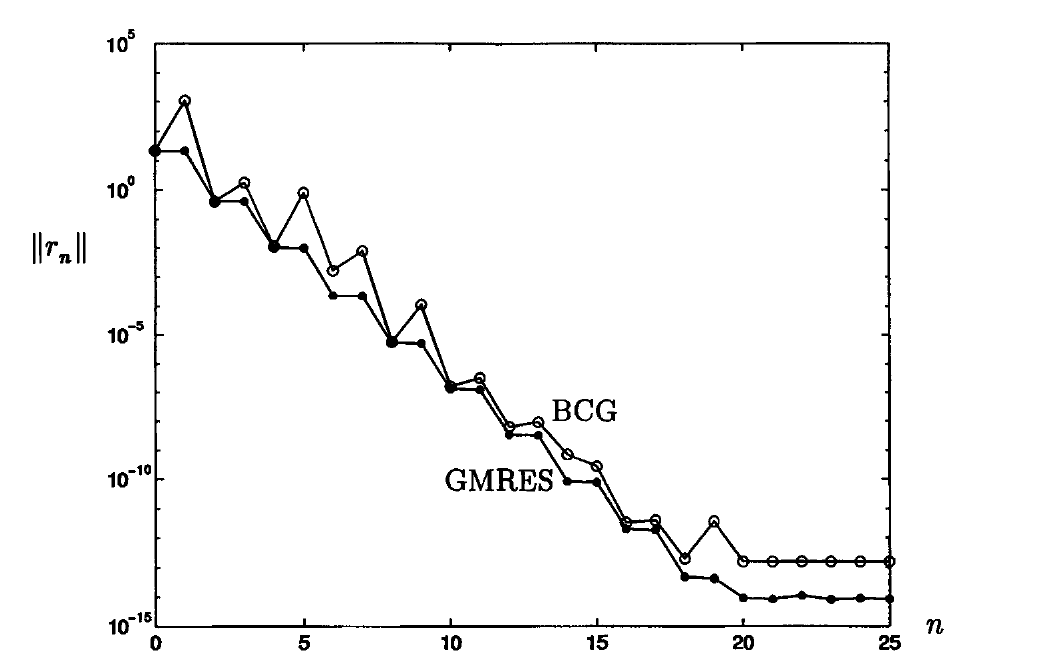
\includegraphics[width=0.82\textwidth]{../assets/figure-39-2-bcg-gmres.png}
\parbox{0.92\textwidth}{\small 图 39.2. 对图 38.1 中标记为 $\tau=0.01$ 的
$500\times500$ 矩阵随机改变所有元素符号后，GMRES 与 BCG 的比较。图中曲线和坐标
标注保留源图形式；正文给出中文解读。}
\end{figure}

图 39.2 的横轴是迭代步数 $n$，它不等于计算代价。每一步 GMRES 需要一次涉及
$A$ 的矩阵--向量乘法，而 BCG 需要分别涉及 $A$ 和 $A^*$ 的乘法。若矩阵--向量
乘法占主要开销且存储空间足够，GMRES 可能因此比 BCG 快一倍甚至更多。不过在本例
中，矩阵足够稀疏，长递推关系的维护开销已经不可忽略；事实上，图 39.2 中 BCG
的计算速度比 GMRES 快两倍以上。

\section*{QMR 及其他变体}

BCG 相对于 GMRES 的一个重要优点是使用三项递推：即使需要很多步，每一步的工作量
和存储需求也能保持在可控范围内。但它有两个缺点。

第一，与 GMRES 随步数通常单调且常常很快的收敛相比，BCG 收敛更慢、也更不规则，
有时会比图 39.2 中显示的情况不规则得多。不规则收敛本身就不理想，而且舍入误差
可能使最终可达到的精度降低（见习题 39.4）。极端情况下会发生迭代崩溃：某个内积
变成零，之后无法继续取得进展，即使原线性系统本身是条件良好的。

第二，BCG 既需要乘以 $A$，也需要乘以 $A^*$。这些乘法在数学上以及计算机体系结构
上的实现方式不同，因此额外负担可能从很小到几乎无法承担不等。

针对这两个问题，自 20 世纪 80 年代起，人们提出了十多种 BCG 变体。下面列出几种
最著名的方法，相关参考文献见本书注释：

\begin{itemize}[leftmargin=2.6em]
\item 前视 Lanczos（Look-ahead Lanczos，Parlett、Taylor 和 Liu，1985）；
\item CGS，即共轭梯度平方（conjugate gradients squared，Sonneveld，1989）；
\item QMR，即拟最小残量（quasi-minimal residuals，Freund 和 Nachtigal，1991）；
\item Bi-CGSTAB，即稳定化 BCG（van der Vorst，1992）；
\item TFQMR，即无转置 QMR（transpose-free QMR，Freund，1993）。
\end{itemize}

这里只作简要说明，不给出细节。

\paragraph{前视 Lanczos。}
当迭代即将崩溃时，不一次只走一步，而是一次走两步或更多步，就可能避免崩溃。
Parlett 等人提出的原始想法后来得到广泛发展，例如被纳入 QMR 作者推荐的算法版本。
可以证明，崩溃现象等价于某个函数的 Padé 逼近表中出现相同元素组成的方块；前视
思想就是一次跨过这些方块。实际计算中不会只检测精确崩溃，还要用适当容差定义
“近崩溃”。

\paragraph{CGS。}
如果把 BCG 的两步以另一种方式合并为一步，使算法被“平方化”，就可以避免乘以
$A^*$。结果是一个“无转置”方法，有时收敛速度最多可达 BCG 的两倍，但收敛的
不规则程度也可能约为两倍。

\paragraph{QMR、Bi-CGSTAB 与 TFQMR。}
三项递推不能用来最小化 $\lVert r_n\rVert_2$，但可以用来最小化另一种依赖数据的
范数；实际中，这个范数通常不会和 $\lVert r_n\rVert_2$ 相差太远。这可能显著
改善收敛曲线的平滑性，并降低舍入误差的影响。Bi-CGSTAB 也会显著平滑 BCG 的
收敛速度；TFQMR 则是 QMR 的一个变体，在保持平滑收敛的同时避免了对 $A^*$ 的需求。

最近的工作试图把三种优点结合到一起：平滑的收敛曲线、用于避免崩溃的前视机制，
以及无转置运算。到目前为止，三者还没有在一个算法中得到完全令人满意的结合；
这个研究方向仍然很年轻。

\section*{习题}

\paragraph{39.1.}
考虑矩阵（39.5）给出的 $m$ 维问题 $Ax=b$。

\begin{enumerate}[label=(\alph*)]
\item 证明所有奇异值都等于 1，并说明这为什么意味着 CGN 一步收敛。
\item 证明所有特征值都是 $m$ 次单位根，并说明这为什么意味着对一般的 $b$，
GMRES 需要 $m$ 步才能收敛。
\item 这个矩阵具有很强的结构，不需要借助特征值或奇异值也能理解其收敛行为。
特别地，对右端项 $b=(1,0,0,\ldots,0)^T$，用初等论证解释为什么 GMRES 需要
$m$ 步才能收敛。
\end{enumerate}

\paragraph{39.2.}
构造一个任意维数 $m$ 的矩阵，具有与习题 39.1 几乎相反的性质：GMRES 两步收敛，
而 CGN 需要 $m$ 步。

\paragraph{39.3.}

\begin{enumerate}[label=(\alph*)]
\item 若 $A$ 是 Hermitian 矩阵，并适当地选择 $s_0$，算法 39.1 会退化为算法
38.1。验证这一说法，并确定合适的 $s_0$。
\item 设 $A$ 是复矩阵，且对称但不是 Hermitian。证明选择另一个 $s_0$ 后，
算法 39.1 仍可退化为只包含一个三项递推的迭代。
\end{enumerate}

\paragraph{39.4.}
图 39.2 表明，如果双正交化方法的收敛曲线含有尖峰，那么它可能影响浮点算术中
最终可达到的精度。不必追求严格证明，解释为什么会这样，并评论它与高斯消去中
增长因子（第 22 讲）的类比。

\paragraph{39.5.}
对于下面的 $m\times m$ 问题 $Ax=b$，你认为 CG、GMRES、CGN、BCG 中哪一个最有效？
说明理由。

\begin{enumerate}[label=(\alph*)]
\item 稠密的非 Hermitian 矩阵，$m=10^4$，除三个特征值外，其余特征值都近似等于 $-1$。
\item 与（a）相同，但除三个特征值外，其余特征值散布在区域
$-10\leq\operatorname{Re}(\lambda)\leq10$、$-1\leq\operatorname{Im}(\lambda)\leq1$。
\item 稀疏的非 Hermitian 矩阵，$m=10^6$，但只有 $10^7$ 个非零元；特征值如（a）。
\item 稀疏的 Hermitian 矩阵，$m=10^5$，特征值散布在区间 $[1,100]$。
\item 与（d）相同，但有两个离群特征值 $0.01$ 和 $10000$。
\item 与（d）相同，但另外还有离群特征值 $-1$、$-10$ 和 $-100$。
\item 稀疏的正规矩阵，$m=10^5$，特征值是复数，散布在环域
$1\leq|\lambda|\leq2$ 内。
\end{enumerate}

\end{document}
